\documentclass[]{elsarticle} %review=doublespace preprint=single 5p=2 column
%%% Begin My package additions %%%%%%%%%%%%%%%%%%%
\usepackage[hyphens]{url}

  \journal{Journal of Gastroenterology} % Sets Journal name


\usepackage{lineno} % add
\providecommand{\tightlist}{%
  \setlength{\itemsep}{0pt}\setlength{\parskip}{0pt}}

\usepackage{graphicx}
\usepackage{booktabs} % book-quality tables
%%%%%%%%%%%%%%%% end my additions to header

\usepackage[T1]{fontenc}
\usepackage{lmodern}
\usepackage{amssymb,amsmath}
\usepackage{ifxetex,ifluatex}
\usepackage{fixltx2e} % provides \textsubscript
% use upquote if available, for straight quotes in verbatim environments
\IfFileExists{upquote.sty}{\usepackage{upquote}}{}
\ifnum 0\ifxetex 1\fi\ifluatex 1\fi=0 % if pdftex
  \usepackage[utf8]{inputenc}
\else % if luatex or xelatex
  \usepackage{fontspec}
  \ifxetex
    \usepackage{xltxtra,xunicode}
  \fi
  \defaultfontfeatures{Mapping=tex-text,Scale=MatchLowercase}
  \newcommand{\euro}{€}
\fi
% use microtype if available
\IfFileExists{microtype.sty}{\usepackage{microtype}}{}
\bibliographystyle{elsarticle-harv}
\usepackage{longtable}
\usepackage{graphicx}
% We will generate all images so they have a width \maxwidth. This means
% that they will get their normal width if they fit onto the page, but
% are scaled down if they would overflow the margins.
\makeatletter
\def\maxwidth{\ifdim\Gin@nat@width>\linewidth\linewidth
\else\Gin@nat@width\fi}
\makeatother
\let\Oldincludegraphics\includegraphics
\renewcommand{\includegraphics}[1]{\Oldincludegraphics[width=\maxwidth]{#1}}
\ifxetex
  \usepackage[setpagesize=false, % page size defined by xetex
              unicode=false, % unicode breaks when used with xetex
              xetex]{hyperref}
\else
  \usepackage[unicode=true]{hyperref}
\fi
\hypersetup{breaklinks=true,
            bookmarks=true,
            pdfauthor={},
            pdftitle={Template for the Creation of Reproducable Research Journal Articles using R Markdown},
            colorlinks=false,
            urlcolor=blue,
            linkcolor=magenta,
            pdfborder={0 0 0}}
\urlstyle{same}  % don't use monospace font for urls

\setcounter{secnumdepth}{0}
% Pandoc toggle for numbering sections (defaults to be off)
\setcounter{secnumdepth}{0}
% Pandoc header
\usepackage{booktabs}
\usepackage{longtable}
\usepackage{array}
\usepackage{multirow}
\usepackage{wrapfig}
\usepackage{float}
\usepackage{colortbl}
\usepackage{pdflscape}
\usepackage{tabu}
\usepackage{threeparttable}
\usepackage{threeparttablex}
\usepackage[normalem]{ulem}
\usepackage{makecell}
\usepackage{xcolor}



\begin{document}
\begin{frontmatter}

  \title{Template for the Creation of Reproducable Research Journal Articles
using R Markdown}
    \author[Some Institute of Technology]{Megan Magee\corref{c1}}
   \ead{mageem@mcmaster.ca} 
   \cortext[c1]{Corresponding Authors}
    \author[Another University]{Philip Britz-McKibbin}
   \ead{britz@mcmaster.ca} 
  
    \author[Again Another University]{Additional Author}
  
  
      \address[Some Institute of Technology]{McMaster University, Department of Chemistry and Chemical Biology, Main
St W, Hamilton, ON, L8S 4L8}
    \address[Another University]{McMaster University, Department of Chemsitry and Chemical Biology, Main
St W, Hamilton, ON, L8S 4L8}
    \address[Again Another University]{McMaster Children's Hospital, Main St W, Hamilton, ON, L8N 3Z5}
  
  \begin{abstract}
  As of late, the need for journal articles to be created in such a way
  that the work done and the data analysis displayed in these articles can
  be reproduced, has become a growing aspect of importance in the research
  industry. Currently, many researchers do not have a definitive practice
  in place that will ensure that their research can be understood and
  recreated by fellow researchers. Without a means of reproducing research
  results, the research process for many researchers may be delayed as
  additional time and money must be spent on attempts to recreate results
  that have already been proven. The purpose of this article is to act as
  a template for the writing of future research papers by the Britz
  McKibbin group in hopes that the document will be easily reproduced by
  future lab members and fellow researchers alike. This article template
  will display the many different possible uses of R along with the
  formatting features that are commonly used by the Britz group and how to
  recreate them with the R Software.
  
  By using the R programming software to write journal articles, all of
  the details related to the displayed statistical analyseies in the
  journal will be avaialble to the reader by looking at the R script.
  These R scripts which will be stored in a GitHub repository, may be
  accessed by the public upon request.
  \end{abstract}
  
 \end{frontmatter}

\hypertarget{keywords}{%
\section{Keywords}\label{keywords}}

LaTex; R Markdown; Reproducable Research

\hypertarget{introduction}{%
\section{Introduction}\label{introduction}}

\hypertarget{background}{%
\paragraph{background}\label{background}}

In this template journal article, we will go through and explain how to
perform statistical analysis and data transformations. The key features
we will discuss include; taking the mean of a dataset variable(s),
performing log transformations, inputing data into simple and complex
tables, how to format tables, introduction of math notation into the
article, plotting simple graphs along with more complex pinciple
component analysis graphs and heat map analysis, as well as figure input
and layout options.

\hypertarget{mean-and-log-transformations}{%
\section{Mean and Log
Transformations}\label{mean-and-log-transformations}}

Taking the mean of a data set is an important data transfermation that
is necessary in research practice before further statistical analysis
can be performed. The same can be said about log transformations. The
purpose in our research for performing a log transformation on our data
set is to create a set of values that are within a smaller range as it
increases the accuracy of statistical analyses that use varience as a
key component for data correlation. This is necessary before you perform
an analysis such as PCA, as highly differential values will skewer PCA
results and often prevent proper clustering.

\hypertarget{mean}{%
\paragraph{mean}\label{mean}}

When taking a mean of a set of data you need to first define the data
set from which you will take the mean. You are not limited to only
taking the mean of the entire data set, you are also able to specify
which rows and columns you want to be included in the mean calculation.
The function \emph{Select}(Column Name:Column Name) will select for the
range of columns specified, while the function \emph{Filter}(Row Name:
Row Name) will select for the specified rows. After the filters have
applied, the \textbf{lapply(mean)} function can be applied to produce
the mean values. By specifying that the columns CF\_1 to CF\_5 of the
CF\_BiomarkersPCA dataset should be included in the mean calculation,
the following values were obtained:

\begin{verbatim}
     CF_1      CF_2      CF_3      CF_4      CF_5 
0.2351090 0.2507217 0.3953087 0.4108190 0.2038396 
\end{verbatim}

When we want to perform a tansformation on a set of data, it may be
required that your data be in a matrix rather then a data frame. In
order to make a matrix of your data set, you want to turn your row
numbers into your labeling variable. In the \textbf{CF\_Biomarkers}
matrix, this would be the ``Label'' variable. Once the row names have
been set, the data set is turned into a matrix using the function
\emph{data.matrix}(Dataset Name)

\hypertarget{log-transformation}{%
\paragraph{log transformation}\label{log-transformation}}

The log transformation of data can be done by first defining what we
want to transform, for example, the relative peak areas (RPA), or
possibly the entire matrix. The transformation is then done by
performing the function \emph{log(Matrix Name)} and assigning a name to
the newly transformed data (e.g T\_logBM)

This will perform the transformation, but in order to visualize it you
must type the new transformed data's name \emph{T\_logBM} in a chunk of
R code. The way that data is displayed in the optput document is not
appealing as it is so we opt. to put the outputted data in a table. In
order to display the table in a way that is appealing and logical, the
two types of patient samples were divided (CF and CF NEG) into separate
tables.

\begin{table}[H]

\caption{\label{tab:visualize log transformation positive}Visualization of Log Transformed Data for CF Positive Patients}
\centering
\resizebox{\linewidth}{!}{
\begin{tabular}[t]{lrrrrrrrrrrrr}
\toprule
Biomarker & CF\_1 & CF\_2 & CF\_3 & CF\_4 & CF\_5 & CF\_6 & CF\_7 & CF\_8 & CF\_9 & CF\_10 & CF\_11 & CF\_12\\
\midrule
\rowcolor{gray!6}  76.0393/0.6639 & -0.907 & -0.839 & 0.105 & 0.095 & -1.038 & -1.193 & -0.847 & -0.832 & 0.042 & 0.042 & -1.023 & -1.122\\
90.055/0.5772 & -3.458 & -3.403 & -3.532 & -3.306 & -3.147 & -3.438 & -3.637 & -3.606 & -3.817 & -3.773 & -3.440 & -3.659\\
\rowcolor{gray!6}  90.055/0.7215 & -0.234 & -0.199 & 1.322 & 1.362 & -0.018 & -0.172 & -0.144 & -0.128 & 1.281 & 1.297 & -0.004 & -0.152\\
104.0706/0.7672 & -3.456 & -3.436 & -3.838 & -3.894 & -4.125 & -4.210 & -3.871 & -3.629 & -3.713 & -3.545 & -3.622 & -3.665\\
\rowcolor{gray!6}  104.0706/0.7718 & -3.358 & -3.045 & -3.097 & -3.145 & -3.012 & -3.077 & -3.212 & -3.239 & -3.127 & -3.266 & -3.054 & -3.059\\
\addlinespace
104.1075/0.5315 & -1.107 & -0.455 & 0.505 & 0.501 & -0.690 & -1.087 & -1.223 & -1.027 & 0.371 & 0.425 & -0.933 & -1.288\\
\rowcolor{gray!6}  106.0499/0.8165 & -1.584 & -1.499 & -0.744 & -0.737 & -1.742 & -1.946 & -1.480 & -1.552 & -0.808 & -0.812 & -1.797 & -1.866\\
113.0346/0.8719 & -4.595 & -4.879 & -4.451 & -4.400 & -5.096 & -5.026 & -4.815 & -4.381 & -4.533 & -4.382 & -4.893 & -4.999\\
\rowcolor{gray!6}  114.0662/0.5721 & -0.861 & -0.701 & -0.752 & -0.740 & -1.243 & -1.323 & -0.739 & -0.713 & -0.936 & -0.916 & -1.400 & -1.403\\
116.0706/0.8871 & -0.140 & -0.090 & 0.449 & 0.494 & -0.163 & -0.202 & -0.002 & -0.003 & 0.440 & 0.405 & -0.132 & -0.160\\
\addlinespace
\rowcolor{gray!6}  118.0611/0.6563 & -4.813 & -4.749 & -4.680 & -4.769 & -5.842 & -5.376 & -4.936 & -4.696 & -4.935 & -4.688 & -5.218 & -5.410\\
118.0863/0.674 & -3.198 & -3.243 & -3.499 & -3.527 & -4.264 & -4.098 & -4.032 & -4.013 & -3.657 & -3.605 & -3.793 & -3.812\\
\rowcolor{gray!6}  118.0863/0.9436 & -0.790 & -0.818 & -0.876 & -0.861 & -1.191 & -1.299 & -0.896 & -0.896 & -1.017 & -1.044 & -1.329 & -1.382\\
120.0655/0.8643 & -1.339 & -1.306 & -0.804 & -0.757 & -1.282 & -1.435 & -1.251 & -1.192 & -0.799 & -0.795 & -1.101 & -1.275\\
\rowcolor{gray!6}  123.0553/0.5961 & -2.427 & -2.242 & -1.388 & -1.360 & -2.091 & -2.318 & -2.414 & -2.354 & -1.531 & -1.513 & -2.042 & -2.241\\
\addlinespace
132.0655/1.0258 & -3.046 & -2.884 & -2.626 & -2.637 & -3.011 & -3.176 & -2.951 & -2.888 & -2.731 & -2.604 & -3.101 & -3.115\\
\rowcolor{gray!6}  132.0768/0.7069 & -0.088 & -0.083 & 0.069 & 0.082 & 0.262 & 0.230 & -0.041 & -0.064 & 0.012 & 0.041 & 0.320 & 0.305\\
132.1019/0.8189 & -0.587 & -0.347 & -1.297 & -0.877 & -0.441 & -1.034 & -0.485 & -0.343 & -1.355 & -1.014 & -0.512 & -1.026\\
\rowcolor{gray!6}  132.1019/0.8305 & 0.307 & 0.138 & 0.064 & 0.085 & -0.249 & -0.319 & 0.412 & 0.181 & -0.026 & 0.028 & -0.294 & -0.341\\
133.0608/0.8644 & -2.545 & -2.440 & -3.752 & -3.976 & -2.576 & -2.454 & -2.259 & -2.160 & -3.531 & -3.499 & -2.004 & -2.165\\
\addlinespace
\rowcolor{gray!6}  133.0972/0.5383 & -1.661 & -1.698 & -1.519 & -1.462 & -1.988 & -2.140 & -1.568 & -1.656 & -1.515 & -1.520 & -1.779 & -1.764\\
134.0448/0.9647 & -2.627 & -2.463 & -4.387 & -4.272 & -3.031 & -2.866 & -2.504 & -2.526 & -4.438 & -4.514 & -2.541 & -2.621\\
\rowcolor{gray!6}  137.0458/1.121 & 0.093 & 0.195 & 1.028 & 1.073 & -4.552 & -3.594 & 0.218 & 0.240 & 1.007 & 0.987 & -4.387 & -3.569\\
144.0988/0.952 & -2.172 & -2.140 & -1.856 & -1.800 & -3.762 & -4.257 & -2.308 & -2.244 & -2.086 & -2.069 & -4.385 & -4.602\\
\rowcolor{gray!6}  146.1176/0.6388 & -3.128 & -3.159 & -3.084 & -3.085 & -3.448 & -3.429 & -3.356 & -3.358 & -3.422 & -3.294 & -3.542 & -3.727\\
\addlinespace
147.0764/0.8941 & -0.146 & -0.092 & -2.232 & -2.283 & -0.248 & -0.226 & -0.020 & -0.037 & -2.385 & -2.346 & -0.088 & -0.102\\
\rowcolor{gray!6}  147.1128/0.5403 & -1.317 & -1.325 & -0.841 & -0.818 & -1.466 & -1.557 & -1.264 & -1.239 & -0.914 & -0.899 & -1.269 & -1.290\\
148.0604/0.9091 & -1.522 & -1.429 & -0.940 & -0.880 & -1.547 & -1.704 & -1.417 & -1.375 & -0.952 & -0.897 & -1.481 & -1.552\\
\rowcolor{gray!6}  150.0583/0.8747 & -3.019 & -2.975 & -2.631 & -2.725 & -3.202 & -3.208 & -2.893 & -2.918 & -2.612 & -2.671 & -3.061 & -3.057\\
156.0768/0.5794 & -1.818 & -1.714 & -1.558 & -1.422 & -1.305 & -1.428 & -1.748 & -1.830 & -1.641 & -1.670 & -1.226 & -1.189\\
\addlinespace
\rowcolor{gray!6}  162.1125/0.6791 & -1.398 & -1.430 & -1.244 & -1.174 & -1.682 & -1.642 & -1.423 & -1.427 & -1.335 & -1.356 & -1.753 & -1.773\\
166.0511/0.9977 & -3.757 & -3.737 & -3.337 & -3.250 & -3.855 & -4.628 & -3.805 & -3.704 & -3.357 & -3.325 & -4.165 & -4.550\\
\rowcolor{gray!6}  166.0511/1.0071 & -3.670 & -3.464 & -3.181 & -3.123 & -3.942 & -4.303 & -3.548 & -3.624 & -3.224 & -3.299 & -4.182 & -4.513\\
166.0863/0.9082 & -0.780 & -0.711 & -0.145 & -0.079 & -0.903 & -1.076 & -0.684 & -0.728 & -0.202 & -0.155 & -0.990 & -1.065\\
\rowcolor{gray!6}  168.0747/0.6301 & -1.994 & -1.958 & -1.157 & -1.098 & -2.952 & -3.175 & -1.863 & -1.851 & -1.168 & -1.167 & -2.912 & -3.130\\
\addlinespace
170.0924/0.5936 & -2.922 & -2.826 & -3.501 & -3.219 & -2.253 & -2.208 & -2.899 & -2.888 & -3.515 & -3.494 & -2.129 & -2.069\\
\rowcolor{gray!6}  175.119/0.5603 & -4.546 & -4.344 & -4.545 & -4.493 & -4.098 & -4.267 & -4.777 & -4.528 & -4.533 & -4.548 & -4.097 & -4.440\\
176.0706/0.6945 & -4.996 & -4.975 & -4.725 & -4.702 & -4.929 & -5.018 & -4.976 & -4.845 & -5.083 & -4.987 & -4.923 & -5.476\\
\rowcolor{gray!6}  176.103/0.9243 & -2.329 & -2.321 & -2.229 & -2.218 & -2.283 & -2.470 & -2.229 & -2.205 & -2.305 & -2.251 & -2.328 & -2.352\\
180.0866/0.7301 & -4.620 & -4.517 & -4.732 & -5.078 & -4.800 & -4.752 & -4.695 & -5.053 & -4.815 & -4.945 & -4.843 & -4.607\\
\addlinespace
\rowcolor{gray!6}  182.0812/0.9476 & -1.800 & -1.686 & -1.417 & -1.389 & -1.885 & -2.045 & -1.672 & -1.637 & -1.400 & -1.397 & -1.719 & -1.899\\
189.1603/0.55 & -4.318 & -4.267 & -4.339 & -4.420 & -4.637 & -4.867 & -4.982 & -5.161 & -5.620 & -5.540 & -4.972 & -5.329\\
\rowcolor{gray!6}  204.123/0.7251 & -2.314 & -2.327 & -2.882 & -2.891 & -1.909 & -1.962 & -2.348 & -2.448 & -3.206 & -3.230 & -2.034 & -2.043\\
205.0972/0.91 & -2.447 & -2.477 & -2.343 & -2.351 & -2.560 & -2.758 & -2.314 & -2.230 & -2.422 & -2.389 & -2.403 & -2.412\\
\rowcolor{gray!6}  218.1387/0.7483 & -4.524 & -4.011 & -5.165 & -4.996 & -4.344 & -4.053 & -4.642 & -4.327 & -5.568 & -5.292 & -4.158 & -3.661\\
\addlinespace
238.0947/1.1082 & -7.149 & -7.149 & -6.827 & -6.827 & -7.088 & -7.088 & -7.011 & -7.011 & -6.951 & -6.951 & -6.701 & -6.701\\
\rowcolor{gray!6}  252.1091/1.1525 & -6.801 & -6.801 & -6.779 & -6.779 & -6.620 & -6.620 & -7.900 & -7.900 & -7.900 & -7.900 & -7.900 & -7.900\\
298.1146/0.843 & -4.615 & -4.477 & -7.266 & -6.699 & -5.240 & -5.112 & -4.740 & -4.451 & -7.235 & -7.417 & -4.965 & -5.054\\
\rowcolor{gray!6}  307.0833/1.0435 & -3.150 & -3.188 & -5.650 & -5.078 & -3.339 & -3.292 & -3.116 & -3.052 & -5.180 & -5.204 & -2.776 & -2.921\\
\bottomrule
\end{tabular}}
\end{table}

\begin{table}[H]

\caption{\label{tab:visualize log transformation negative}VIsualization of Log Transformed Data for CF Negative Patients}
\centering
\resizebox{\linewidth}{!}{
\begin{tabular}[t]{lrrrrrrrrrrrr}
\toprule
Biomarker & NEG\_1 & NEG\_2 & NEG\_3 & NEG\_4 & NEG\_5 & NEG\_6 & NEG\_7 & NEG\_8 & NEG\_9 & NEG\_10 & NEG\_11 & NEG\_12\\
\midrule
\rowcolor{gray!6}  76.0393/0.6639 & -1.654 & -1.607 & -1.683 & -1.683 & -1.679 & -1.678 & -1.822 & -1.773 & -1.640 & -1.694 & -1.618 & -1.725\\
90.055/0.5772 & -4.022 & -3.989 & -4.003 & -3.857 & -3.866 & -4.041 & -4.254 & -3.974 & -4.114 & -4.059 & -3.836 & -4.126\\
\rowcolor{gray!6}  90.055/0.7215 & -0.346 & -0.252 & -0.257 & -0.294 & -0.230 & -0.383 & -0.545 & -0.437 & -0.265 & -0.288 & -0.233 & -0.340\\
104.0706/0.7672 & -3.749 & -3.926 & -3.722 & -3.766 & -3.706 & -3.654 & -3.787 & -3.625 & -4.257 & -3.866 & -3.750 & -3.764\\
\rowcolor{gray!6}  104.0706/0.7718 & -3.511 & -3.616 & -4.030 & -3.998 & -4.161 & -4.302 & -3.443 & -3.447 & -4.046 & -3.973 & -3.937 & -4.003\\
\addlinespace
104.1075/0.5315 & -1.552 & -1.360 & -1.222 & -1.261 & -1.122 & -1.147 & -1.268 & -1.133 & -1.194 & -1.203 & -0.983 & -1.143\\
\rowcolor{gray!6}  106.0499/0.8165 & -2.002 & -1.934 & -2.517 & -2.466 & -2.353 & -2.345 & -1.972 & -1.958 & -2.329 & -2.279 & -1.970 & -2.055\\
113.0346/0.8719 & -4.908 & -4.929 & -4.898 & -4.708 & -4.782 & -4.756 & -4.628 & -4.899 & -4.876 & -4.700 & -4.909 & -4.705\\
\rowcolor{gray!6}  114.0662/0.5721 & -0.902 & -0.823 & -0.588 & -0.541 & -0.563 & -0.636 & -1.170 & -1.211 & -0.723 & -0.690 & -0.697 & -0.764\\
116.0706/0.8871 & 0.022 & 0.057 & -0.384 & -0.453 & -0.384 & -0.421 & -0.135 & -0.084 & -0.400 & -0.391 & -0.381 & -0.436\\
\addlinespace
\rowcolor{gray!6}  118.0611/0.6563 & -5.163 & -5.041 & -4.608 & -4.637 & -4.789 & -4.803 & -5.230 & -5.233 & -4.670 & -4.697 & -4.982 & -4.702\\
118.0863/0.674 & -3.656 & -3.488 & -3.423 & -3.515 & -3.460 & -3.686 & -3.568 & -3.625 & -3.920 & -4.038 & -4.119 & -3.991\\
\rowcolor{gray!6}  118.0863/0.9436 & -1.000 & -1.000 & -0.921 & -0.933 & -0.920 & -0.952 & -1.156 & -1.156 & -0.864 & -0.837 & -0.838 & -0.919\\
120.0655/0.8643 & -1.630 & -1.563 & -2.009 & -1.981 & -1.708 & -1.865 & -1.682 & -1.678 & -1.864 & -1.877 & -1.624 & -1.817\\
\rowcolor{gray!6}  123.0553/0.5961 & -2.303 & -2.122 & -2.148 & -2.207 & -2.343 & -2.330 & -2.675 & -2.312 & -2.331 & -2.578 & -2.337 & -2.644\\
\addlinespace
132.0655/1.0258 & -3.500 & -3.588 & -3.411 & -3.369 & -3.175 & -3.320 & -3.631 & -3.495 & -3.247 & -3.347 & -3.222 & -3.216\\
\rowcolor{gray!6}  132.0768/0.7069 & 0.576 & 0.509 & 0.176 & 0.164 & 0.205 & 0.154 & 0.244 & 0.251 & 0.126 & 0.111 & 0.123 & 0.082\\
132.1019/0.8189 & -0.721 & -0.660 & -1.261 & -1.222 & -0.944 & -1.200 & -0.907 & -0.796 & -1.207 & -1.180 & -1.064 & -1.194\\
\rowcolor{gray!6}  132.1019/0.8305 & 0.039 & -0.123 & -0.388 & -0.391 & -0.395 & -0.440 & -0.252 & -0.281 & -0.399 & -0.406 & -0.373 & -0.437\\
133.0608/0.8644 & -2.339 & -2.320 & -3.247 & -3.404 & -3.024 & -3.134 & -2.188 & -2.069 & -2.803 & -2.862 & -2.817 & -2.753\\
\addlinespace
\rowcolor{gray!6}  133.0972/0.5383 & -2.257 & -2.133 & -3.225 & -3.151 & -2.669 & -2.626 & -2.197 & -2.172 & -2.774 & -2.748 & -2.464 & -2.570\\
134.0448/0.9647 & -2.091 & -2.021 & -2.504 & -2.571 & -2.135 & -2.266 & -2.123 & -2.030 & -2.339 & -2.353 & -2.053 & -2.079\\
\rowcolor{gray!6}  137.0458/1.121 & -5.718 & -5.718 & -2.983 & -2.975 & -2.979 & -3.168 & -5.962 & -5.962 & -2.913 & -3.041 & -2.979 & -3.002\\
144.0988/0.952 & -2.521 & -2.510 & -3.063 & -3.049 & -3.111 & -3.018 & -2.640 & -2.597 & -2.920 & -2.925 & -3.017 & -3.049\\
\rowcolor{gray!6}  146.1176/0.6388 & -3.035 & -2.962 & -3.135 & -3.168 & -3.266 & -3.142 & -3.296 & -3.222 & -3.193 & -3.219 & -3.084 & -3.151\\
\addlinespace
147.0764/0.8941 & -0.019 & -0.043 & -0.369 & -0.372 & -0.189 & -0.237 & -0.061 & -0.041 & -0.189 & -0.191 & -0.188 & -0.212\\
\rowcolor{gray!6}  147.1128/0.5403 & -1.878 & -1.825 & -2.711 & -2.677 & -2.349 & -2.428 & -1.776 & -1.829 & -2.488 & -2.473 & -2.340 & -2.481\\
148.0604/0.9091 & -1.436 & -1.403 & -1.105 & -1.126 & -0.847 & -0.863 & -1.316 & -1.310 & -0.851 & -0.836 & -0.733 & -0.828\\
\rowcolor{gray!6}  150.0583/0.8747 & -2.801 & -2.726 & -4.075 & -4.262 & -3.571 & -3.834 & -2.848 & -2.961 & -3.855 & -3.715 & -3.710 & -3.803\\
156.0768/0.5794 & -1.688 & -1.659 & -2.353 & -2.316 & -1.963 & -2.012 & -1.788 & -1.718 & -2.021 & -2.096 & -1.996 & -2.092\\
\addlinespace
\rowcolor{gray!6}  162.1125/0.6791 & -1.497 & -1.488 & -1.638 & -1.676 & -1.612 & -1.705 & -1.760 & -1.736 & -1.689 & -1.674 & -1.739 & -1.705\\
166.0511/0.9977 & -4.073 & -4.147 & -4.212 & -3.907 & -3.963 & -4.081 & -4.406 & -4.686 & -4.162 & -3.927 & -3.984 & -4.204\\
\rowcolor{gray!6}  166.0511/1.0071 & -4.074 & -3.615 & -3.896 & -4.036 & -3.699 & -3.938 & -4.027 & -4.129 & -4.059 & -3.889 & -3.812 & -4.143\\
166.0863/0.9082 & -0.979 & -0.964 & -1.374 & -1.369 & -1.242 & -1.350 & -1.110 & -1.149 & -1.302 & -1.317 & -1.310 & -1.355\\
\rowcolor{gray!6}  168.0747/0.6301 & -2.956 & -2.937 & -2.294 & -2.289 & -2.168 & -2.217 & -2.910 & -2.843 & -2.108 & -2.134 & -1.962 & -2.128\\
\addlinespace
170.0924/0.5936 & -3.369 & -3.329 & -3.616 & -3.500 & -3.231 & -3.433 & -3.508 & -3.461 & -3.462 & -3.326 & -3.513 & -3.409\\
\rowcolor{gray!6}  175.119/0.5603 & -3.630 & -3.444 & -4.047 & -4.099 & -3.654 & -3.826 & -3.682 & -3.675 & -4.076 & -3.846 & -3.633 & -3.918\\
176.0706/0.6945 & -5.760 & -5.592 & -5.918 & -5.542 & -5.369 & -5.589 & -5.335 & -5.634 & -5.546 & -5.731 & -5.619 & -6.250\\
\rowcolor{gray!6}  176.103/0.9243 & -2.669 & -2.580 & -2.943 & -2.843 & -2.653 & -2.661 & -2.618 & -2.455 & -2.564 & -2.578 & -2.491 & -2.584\\
180.0866/0.7301 & -2.882 & -2.837 & -3.286 & -3.300 & -2.876 & -2.984 & -2.944 & -2.842 & -2.831 & -2.945 & -2.766 & -2.900\\
\addlinespace
\rowcolor{gray!6}  182.0812/0.9476 & -1.861 & -1.733 & -2.109 & -2.104 & -1.803 & -1.904 & -1.755 & -1.625 & -1.756 & -1.851 & -1.667 & -1.657\\
189.1603/0.55 & -4.457 & -4.318 & -4.454 & -4.515 & -4.602 & -4.800 & -4.793 & -4.996 & -5.507 & -5.523 & -4.920 & -5.218\\
\rowcolor{gray!6}  204.123/0.7251 & -1.824 & -1.755 & -2.233 & -2.317 & -2.204 & -2.367 & -2.088 & -2.102 & -2.221 & -2.290 & -2.326 & -2.396\\
205.0972/0.91 & -3.130 & -3.111 & -3.609 & -3.538 & -3.166 & -3.144 & -3.011 & -2.873 & -3.141 & -3.128 & -2.802 & -3.046\\
\rowcolor{gray!6}  218.1387/0.7483 & -3.176 & -2.921 & -4.041 & -4.413 & -3.912 & -4.172 & -3.519 & -3.478 & -4.592 & -4.537 & -4.528 & -4.547\\
\addlinespace
238.0947/1.1082 & -3.746 & -3.708 & -3.988 & -4.023 & -3.538 & -3.542 & -3.592 & -3.551 & -3.423 & -3.622 & -3.534 & -3.445\\
\rowcolor{gray!6}  252.1091/1.1525 & -3.548 & -3.396 & -3.538 & -3.518 & -3.145 & -3.118 & -3.395 & -3.266 & -3.143 & -3.052 & -2.973 & -3.141\\
298.1146/0.843 & -5.273 & -5.313 & -5.798 & -6.146 & -5.439 & -5.656 & -5.381 & -5.178 & -5.922 & -5.653 & -4.999 & -5.677\\
\rowcolor{gray!6}  307.0833/1.0435 & -3.354 & -3.273 & -3.992 & -4.044 & -3.560 & -3.625 & -3.040 & -3.007 & -3.494 & -3.481 & -3.278 & -3.226\\
\bottomrule
\end{tabular}}
\end{table}

\hypertarget{simple-and-complex-tables}{%
\section{Simple and Complex Tables}\label{simple-and-complex-tables}}

\hypertarget{simple-tables}{%
\paragraph{simple tables}\label{simple-tables}}

Tables can be created very simply by inputting the names of the
different headers/variables and listing the corresponding values below.
This method requires that the user inputs the data manually and produces
a table that can not be readily formatted. These kinds of tables do not
need to be enclosed in a chunk of code as they are a result of R
Markdown formatting features and not an output of a written code. The
following is an example of such table:

\begin{center}
Table 3: Simple table example
\end{center}

\begin{longtable}[]{@{}ll@{}}
\toprule
Sample & Mean\tabularnewline
\midrule
\endhead
CF\_1 & 0.2351090\tabularnewline
CF\_2 & 0.2507217\tabularnewline
CF\_3 & 0.3953087\tabularnewline
CF\_4 & 0.4108190\tabularnewline
CF\_5 & 0.2038396\tabularnewline
\bottomrule
\end{longtable}

As seen above in Table 3, the caption is centered. Centering a caption
or any written text is done by using raw LaTeX in R Markdown (Stack
Overflow (2014))

\hypertarget{complex-tables}{%
\paragraph{complex tables}\label{complex-tables}}

It is also possible to create more complex tables that are susceptable
to a wide range of formatting options. Complex tables are often created
using a data set that has had various statistical functions applied.

\begin{table}[!h]

\caption{\label{tab:descriptive stats}Stat analysis results for dataset}
\centering
\resizebox{\linewidth}{!}{
\begin{tabular}[t]{lrr}
\toprule
Statistic & Relative.migration.time & Relative.peak.area\\
\midrule
\rowcolor{gray!6}  Mean & 0.6993 & 0.3260\\
Max & 0.1130 & 0.5702\\
\rowcolor{gray!6}  Standard Deviation & 0.8719 & 3.9055\\
\bottomrule
\end{tabular}}
\end{table}

The table above has been formatted to include grey stripes on
alternating rows; this feature allows for the reader to more easily
distinguish between rows of data. This feature is esspecially useful for
tables containing a large number of rows and columns. The table has also
been formatted to show only the first 4 digits of each value, which
allows for only the significant digits to be displayed. Other formatting
features included in ths table include the ``scale\_down'' parameter and
Booktabs = TRUE. These features make sure the table is scaled in such a
way that all of the table is fitted between the margins of the paper and
for applying formatting adjustments to create a publication quality
table respectivly.

\hypertarget{math-notation-using-latex}{%
\section{Math Notation using LaTeX}\label{math-notation-using-latex}}

\hypertarget{math-notation}{%
\paragraph{math notation}\label{math-notation}}

R Markdown on its own can perform mathematical calculations by inputting
functions and equations into chunks of code. Although it can calculate
results, it cannot display the equations used in the calculations in a
mathematical notation. In order to display mathematical equations that
are in the proper notation, the package \textbf{LaTeX} is needed. How
LaTeX works is that any equations or symbols inputted between a pair of
string signs (\$) will output the characters in mathematical notation
inline with your text.

By typing \textbf{\$ \(x + 1\) \$} you will get the output : \(x+1\)

Knowing how to input mathematical notation is only the fist step. It is
also important to know how to arrange your equations and thier
respective outputs. if you want your equations in one chunk, but spread
out onto separate lines, you can input backslashes or an align function
to move the equation that follows on to the next line:

\begin{align*}
x + y = z\\
x - y > z\\
x  y < z
\end{align*}

Once your equations are made you will want to add labels to your
equations so that you can reference them throughout the jornal article.
This is done by first introducing the equation with a \emph{begin}
function, then inputting the equation and the label, and finally closing
off the reference with an \emph{end} function.

\begin{equation}
\label{eq:1}
v_{ep}=\mu_{ep}E
\end{equation}

It is now possible to reference this equation we just made using LaTex.
``Equation (\ref{eq:1}) is an example of an equation used in Capillary
Electrophoresis to calculate the \emph{electrophoretic velocity}''.

\hypertarget{plotting-and-arranging}{%
\section{Plotting and Arranging}\label{plotting-and-arranging}}

\hypertarget{plotting}{%
\paragraph{plotting}\label{plotting}}

One of the advantages of R Markdown is that the figures/plots can be
created in R. By having your plots created directly in R Markdown,
recreating the plots becomes very simple. All of the R script that was
used to create the output graph, and all of the formatting and data
processing done to the data to acheive the final figure is available. By
making this information available, the reproducability of the work shown
in the journal article is substantially increased.

If we wanted to visualize the amounts of a certain disease biomarker
present in patient samples, a bar graph could be made. This graph would
have the concentration (RPA) displayed on the Y axis and the sample
labels on the X axis with the relative heights showing the greater or
lesser presence of the specified marker. In order to use our current
data set to do this, we will first have to filter for the biomarker we
want to look at.

Once the data has been filtered, the graph can be created using the
\emph{ggplot} function, coupled with the formatting parameter
\emph{geom\_bar}:

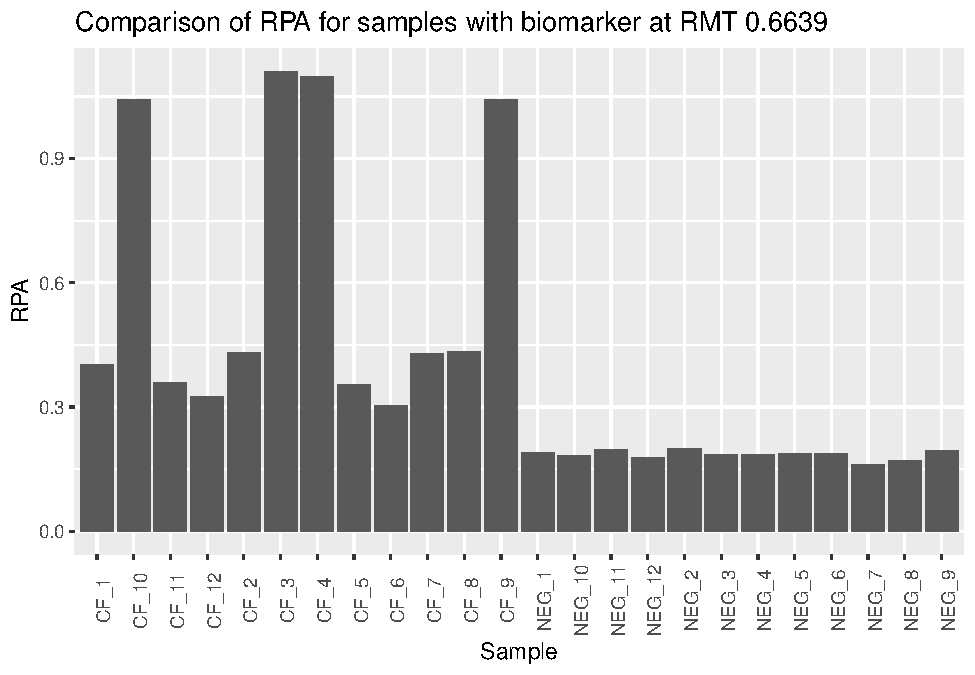
\includegraphics{06DecFinalDeliverableArticle_files/figure-latex/creating the filtered bar graph, fig2-1.pdf}

\hypertarget{arranging-figures}{%
\paragraph{arranging figures}\label{arranging-figures}}

Once the plots have been created you can use either the
\textbf{grid.arrange} or the \textbf{plot\_grid} functions to arrange
your plots so that they appear in one panel or one image. For this paper
we will be placing the bar graph above the scatter plot. By having
multiple figures in one image it becomes easier to compare and analyse
related results.

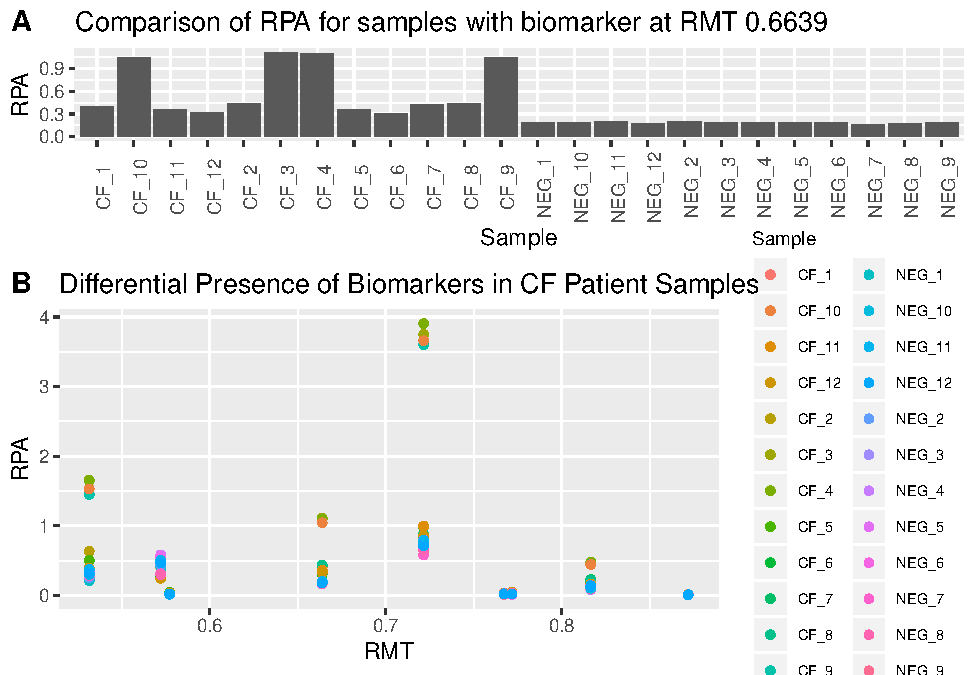
\includegraphics{06DecFinalDeliverableArticle_files/figure-latex/arranginf plots into figure-1.pdf}
Complex Statistical Analysis ============================

\hypertarget{heatmaps}{%
\paragraph{heatmaps}\label{heatmaps}}

Available with R are several packages that allow for the creation of
heatmaps. Depending on which package you use for heatmap generation, it
is possible that the final figure may be slightly different depending on
what kind of transformations are possible with each heatmap function.
Two possible heat map functions include \textbf{heatmap} or
\textbf{heatmap.2} which are functions found within the package
\emph{gplots}. Heatmaps are a useful tool for data visualization, but do
not provide accurate or specific data correlation information.

In order to build a heatmap in R you will need to turn your dataset into
a data matrix. This will ensure the table consists of only results and
there are no variables or headers being included as a value during
analysis. In this paper as explained earlier, the dataset
CF\_BiomarkersPCA was turned into a matrix called Biomarkers\_Matrix.
Although the matrix worked as is, the layout included a row with values
marked as NA, as this is the row that contained the biomarker
\emph{Lable} values. In order to create a more suitable matrix, the
\emph{Label} row was removed from the matrix and the label values were
used to name each of the rows in the Matrix.

Once this was done, a heatmap could be created using the \emph{heatmap}
function:

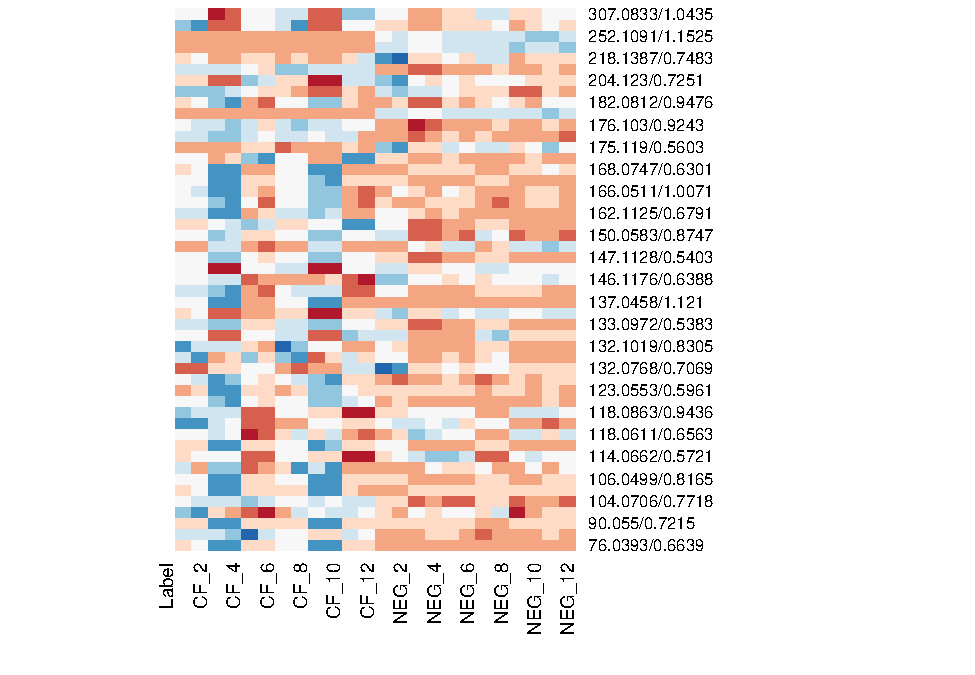
\includegraphics{06DecFinalDeliverableArticle_files/figure-latex/unnamed-chunk-4-1.pdf}
The issue with using this function to create a heatmap is that it does
not have a function that allows a color key to be created. If we want to
include a color key, a more complete heatmap function must be used.

A heatmap was created to include a color key (Row Z-Score) using the
\emph{heatmap.2} function:

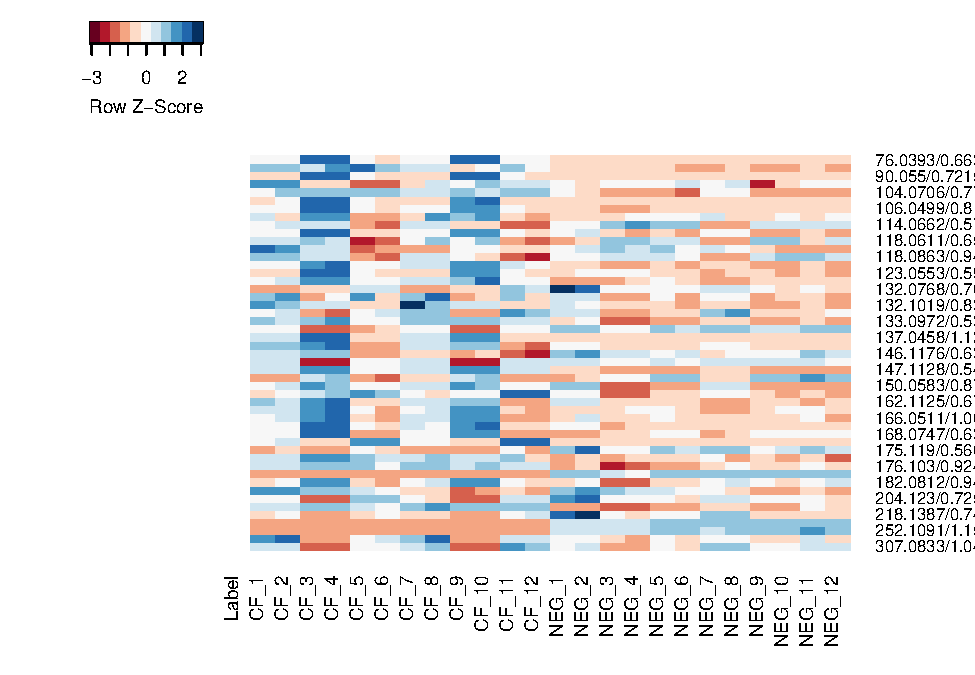
\includegraphics{06DecFinalDeliverableArticle_files/figure-latex/unnamed-chunk-5-1.pdf}

With the way these heatmps were created, the R software does not
recognize them as images, and thus will not allow for the heat maps to
be arranged together into one image as was done earlier with the bar and
scatter plots. To overcome this issue, we can use the function
\textbf{ggplot} which will register the output as a graphical object. In
order to make the plot look like a heat map, rather then a scatter plot,
we can also incorporate the function \emph{geom\_tile} which will plot
the data as tiles, rather then data points.

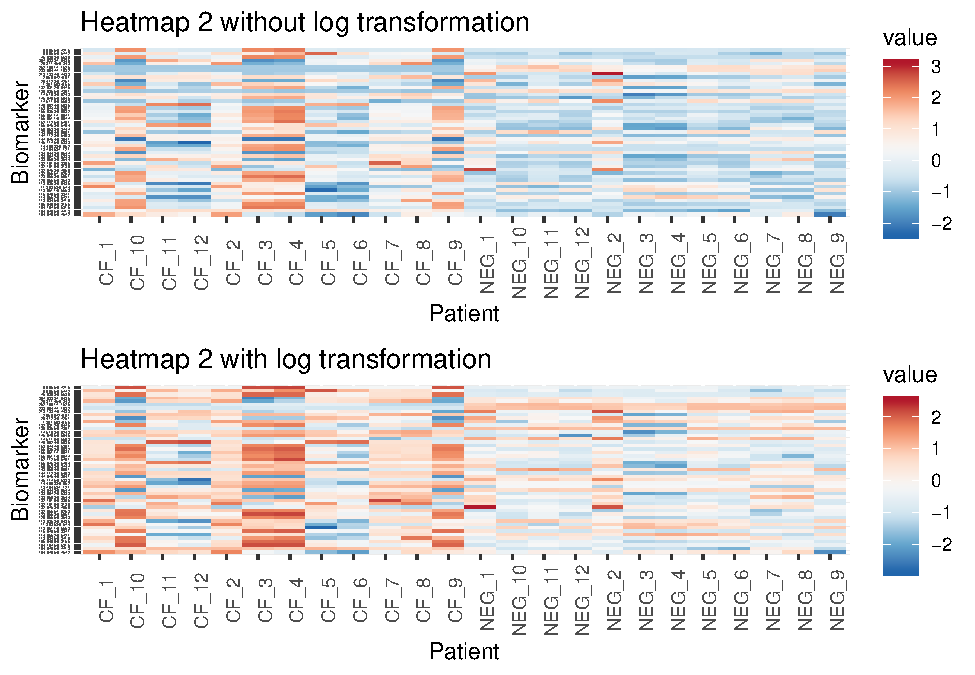
\includegraphics{06DecFinalDeliverableArticle_files/figure-latex/unnamed-chunk-10-1.pdf}

\hypertarget{principle-component-analysis}{%
\paragraph{Principle Component
Analysis}\label{principle-component-analysis}}

Principle component analysis (PCA) is a statistical tool that correlates
and transforms a large number (greater then 2) of variables, into a
smaller set of variables called priciple components. These components
can then be plotted and visualized. Based on how well components group
together you can draw conclusions on which variables may correspond to
certain attributes for each sample. For example, with biomarker
research, you can find that a set of samples that come from patients
carrying a disease will be grouped together, while the set of samplles
taken from healthy individuals will also likely group together based on
their relative abundances of certain biomarkers of disease. As this is a
very important satistical tool for researchers, this article will cover
how to perform this form of data analysis.

For PCA, a data matrix, opposed to a data set is required. For this
example we have the \textbf{CF\_BiomarkerPCA} dataset that has been
turned into a matrix (Biomarker\_Matrix). Before this Matrix can be
used, the data also needs to be log transformed (T\_logBM)

Once the data has been transformed, using the function
\textbf{MetaboAnalystR} we can determine what all of the principle
components are. Once we have the PCs, we plot this information into a
Screeplot and a cumulative variance plot to determine which princile
components hold the greatest varience and which components have a
substantial impact on the clustering of data,

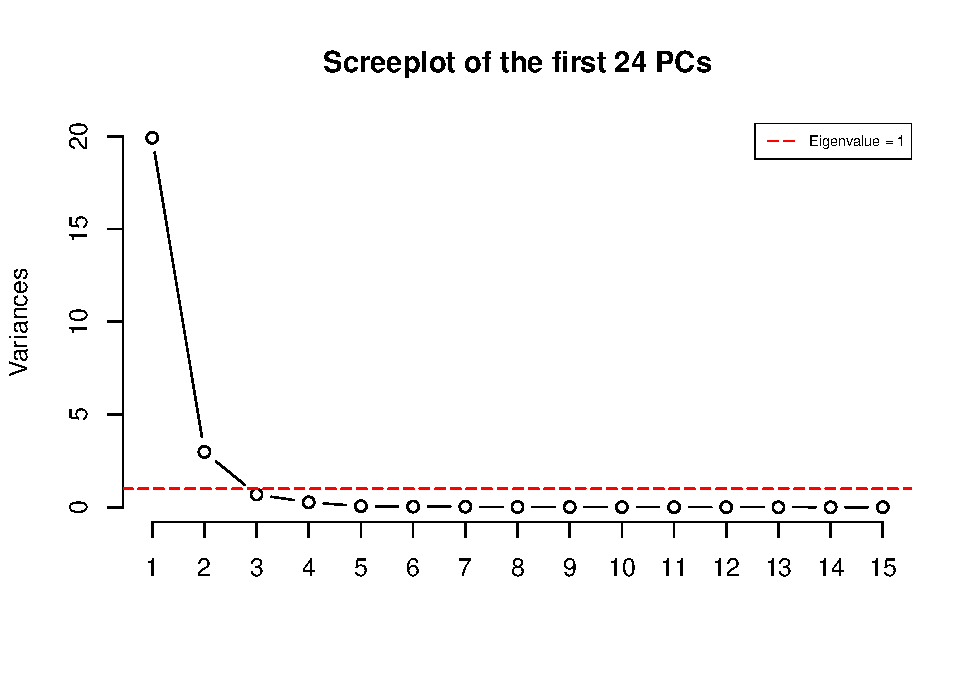
\includegraphics{06DecFinalDeliverableArticle_files/figure-latex/unnamed-chunk-13-1.pdf}

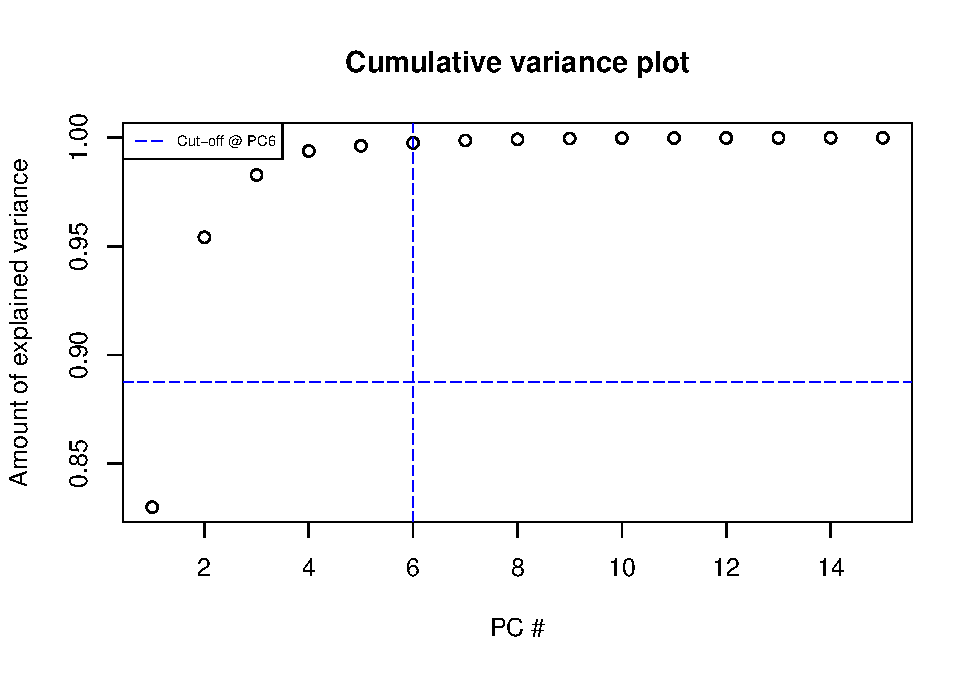
\includegraphics{06DecFinalDeliverableArticle_files/figure-latex/unnamed-chunk-14-1.pdf}

Once you have the background information for your data (Sreeplot and
Cumulative variance plot), you can build your PCA plot. For this
example, we have created a 3D PCA plot by using the functions provided
by the MetaboAnalystR package.

\begin{figure}
\centering
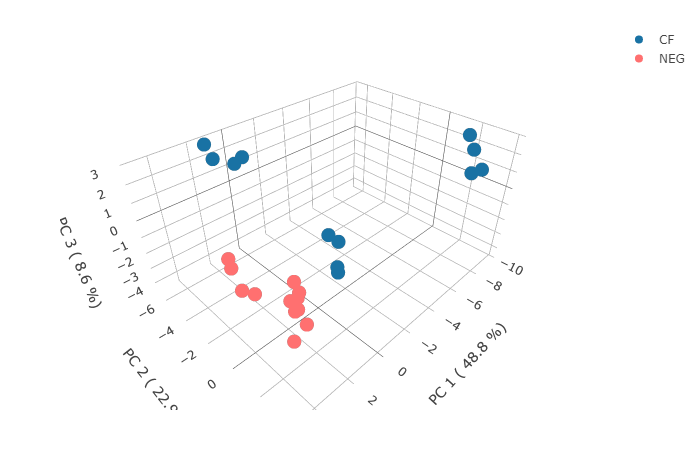
\includegraphics{/Users/megan/Documents/Reproducable research/R/Final Deliverable/FinalDeliverable/newplot.png}
\caption{figure caption here}
\end{figure}

\hypertarget{conclusion}{%
\section{Conclusion}\label{conclusion}}

This template has provided insight into the required functions and
packages for the construction of a basic journal article. The
information and formatting used in this article will stand as a
reference point for all future articles generated in the Britz lab. The
last topic to be covered includes the bibliography and references
sections. If references were used in the article you would reference
them as so Strimbu and Tavel (2010). This reference was obtained from
Google scholar and pasted into the BibTeX file associated with this
template. If manually inputting data into the BibTeX file, follow the
documentation format provided in the origonal BibTeX source document.

\hypertarget{references}{%
\section*{References}\label{references}}
\addcontentsline{toc}{section}{References}

\hypertarget{refs}{}
\leavevmode\hypertarget{ref-Jonathan2014Stack}{}%
Stack Overflow, 2014. Centering image and text in R Markdown for a PDF
report {[}WWW Document{]}. URL
\url{https://stackoverflow.com/questions/24677642/centering-image-and-text-in-r-markdown-for-a-pdf-report}
(accessed 12.10.2019).

\leavevmode\hypertarget{ref-strimbu2010biomarkers}{}%
Strimbu, K., Tavel, J.A., 2010. What are biomarkers? Current Opinion in
HIV and AIDS 5, 463.


\end{document}


